


\begin{document}
This report describes the design, construction, and analysis of an discrete component operational amplifier. The topology chosen includes a simple current mirror that sinks current to a resistively loaded amplifier which in turn is cascaded with an actively loaded differential pair which outputs single-endedly to a common source amplifier stage. This common source stage is then passed to an output Bipolar Junction Transistor (BJT) amplifier stage. The general schematic for a generic op amp is shown in Figure \ref{fig:gen_schem}.

\begin{figure}[H]
    \begin{center}
    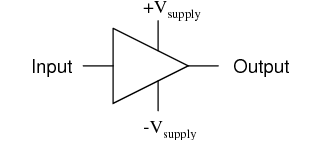
\includegraphics[scale=.35]{Introduction/genericopamp.png}
    \caption{General operational amplifier symbol \cite{b1}}
    \cite{b1}
    \label{fig:gen_schem}
    \end{center}
    
\end{figure}

Operation amplifiers serve an integral building block for modern electronics. Op amps provide large gain with various configuration schema. This allows the circuit designer to use the op amp in different topologies and achieve different results, all without modifying the op amp circuit itself. In addition, an op amp provides significant gain while maintaining stability. The objective of this lab is to create an op amp out of discrete components that achieves the specifications as seen in Table \ref{tab:labspecs}.


\begin{table}[H]
\centering
\caption{Specifications}
\label{tab:labspecs}
\begin{tabular}{|l|l|}
\hline
\textbf{Specifications} &                 \\ \hline
Power                   & $\pm$5V         \\ \hline
Bias Current            & 500 $\mu$A      \\ \hline
Overall Voltage Gain    & 200V/V (46 dB)  \\ \hline
CMRR                    & $\geq$ 60dB     \\ \hline
Output Voltage Swing    & $\geq$ $\pm$ 2V \\ \hline
\end{tabular}
\end{table}

The input stage of an operational amplifier consists of a differential amplifier. For the purposes of this experiment, the NMOS MOSFET that will be used is the ALD1106, and the ALD1107 for the PMOS MOSFET. Differential amplifiers are
desirable for their increased immunity to noise and that DC coupling of stages is possible without
disturbing bias conditions. Each one of these designs will have some
advantage as well as some disadvantage over the other circuits. The primary function of the input
differential pair will be to provide a high common mode rejection ratio (CMRR). The differential gain,
Ad, need not be high, as long as the common mode gain, Acm, is very small. Some op-amp designs use multiple differential input-differential output
stages until they convert to a single ended input.


These differential amplifiers are biased by a current mirror, cascoded or simple, (assumed to be ideal for simulations) and constructed using PMOS and NMOS integrated circuits. The circuit on the left is a resistively loaded differential amplifier. The circuit depicted on the right is an actively loaded differential amplifier. 


\noindent Section 2 of this report describes the design, and when relevant, the simulations of the experiments. Experimental results and implementation are addressed in Section 3. A discussion of the results, sources of error, and areas of possible improvement are outlined in Section 4. Section 5 concludes this report. \newline

\end{document}